
\subsection{Background}
    \textit{Satisfiability Modulo Theories (SMT)} is the problem of determining whether a
    mathematical formula is satisfiable. It generalizes the Boolean satisfiability problem (SAT) to
    more complex formulas involving real numbers, integers, and/or various data structures such as 
    lists, arrays, bit vectors, and strings.

% % % % % % % % % % % % % % % % % % % % % % % % % % % % % % % % % % % % % % % % % % % % % % % % % %

\subsection{Formulation}
    In order to write a proper SMT formulation, we started from the SAT formulation (available in
    the Section \ref{chapter:SAT}) and we have replaced each boolean representation of integer 
    operators with the operators themself.\\

    In particular, the following replacements have been done:
    \begin{align*}
      \text{SMT} \ &\ \leftarrow\ \text{SAT}      \\
                 \cline{1-2}
        a \geq 1 \ &\ \leftarrow\ \text{at\_least\_one}(a) \\
        a \leq 1 \ &\ \leftarrow\ \text{at\_most\_one}(a)  \\
           a = 1 \ &\ \leftarrow\ \text{exactly\_one}(a)   \\
           a = b \ &\ \leftarrow\ \text{equal}(a,b)        \\
           a < b \ &\ \leftarrow\ lt(a,b)                  \\
        a \leq b \ &\ \leftarrow\ lte(a,b)                 \\
           a > b \ &\ \leftarrow\ gt(a,b)                  \\
        a \geq b \ &\ \leftarrow\ gte(a,b)                 \\
           a + b \ &\ \leftarrow\ sum\_b(a,b)              \\   
           a - b \ &\ \leftarrow\ sub\_b(a,b)                 
    \end{align*}

    The final formulation obtained is very "near" to the one defined for CP in the
    Section \ref{chapter:CP}.

% % % % % % % % % % % % % % % % % % % % % % % % % % % % % % % % % % % % % % % % % % % % % % % % % %

\subsection{Results}
    \colorbox{BurntOrange}{TODO missing ...} \\

    \begin{figure}[H]
      \centering
      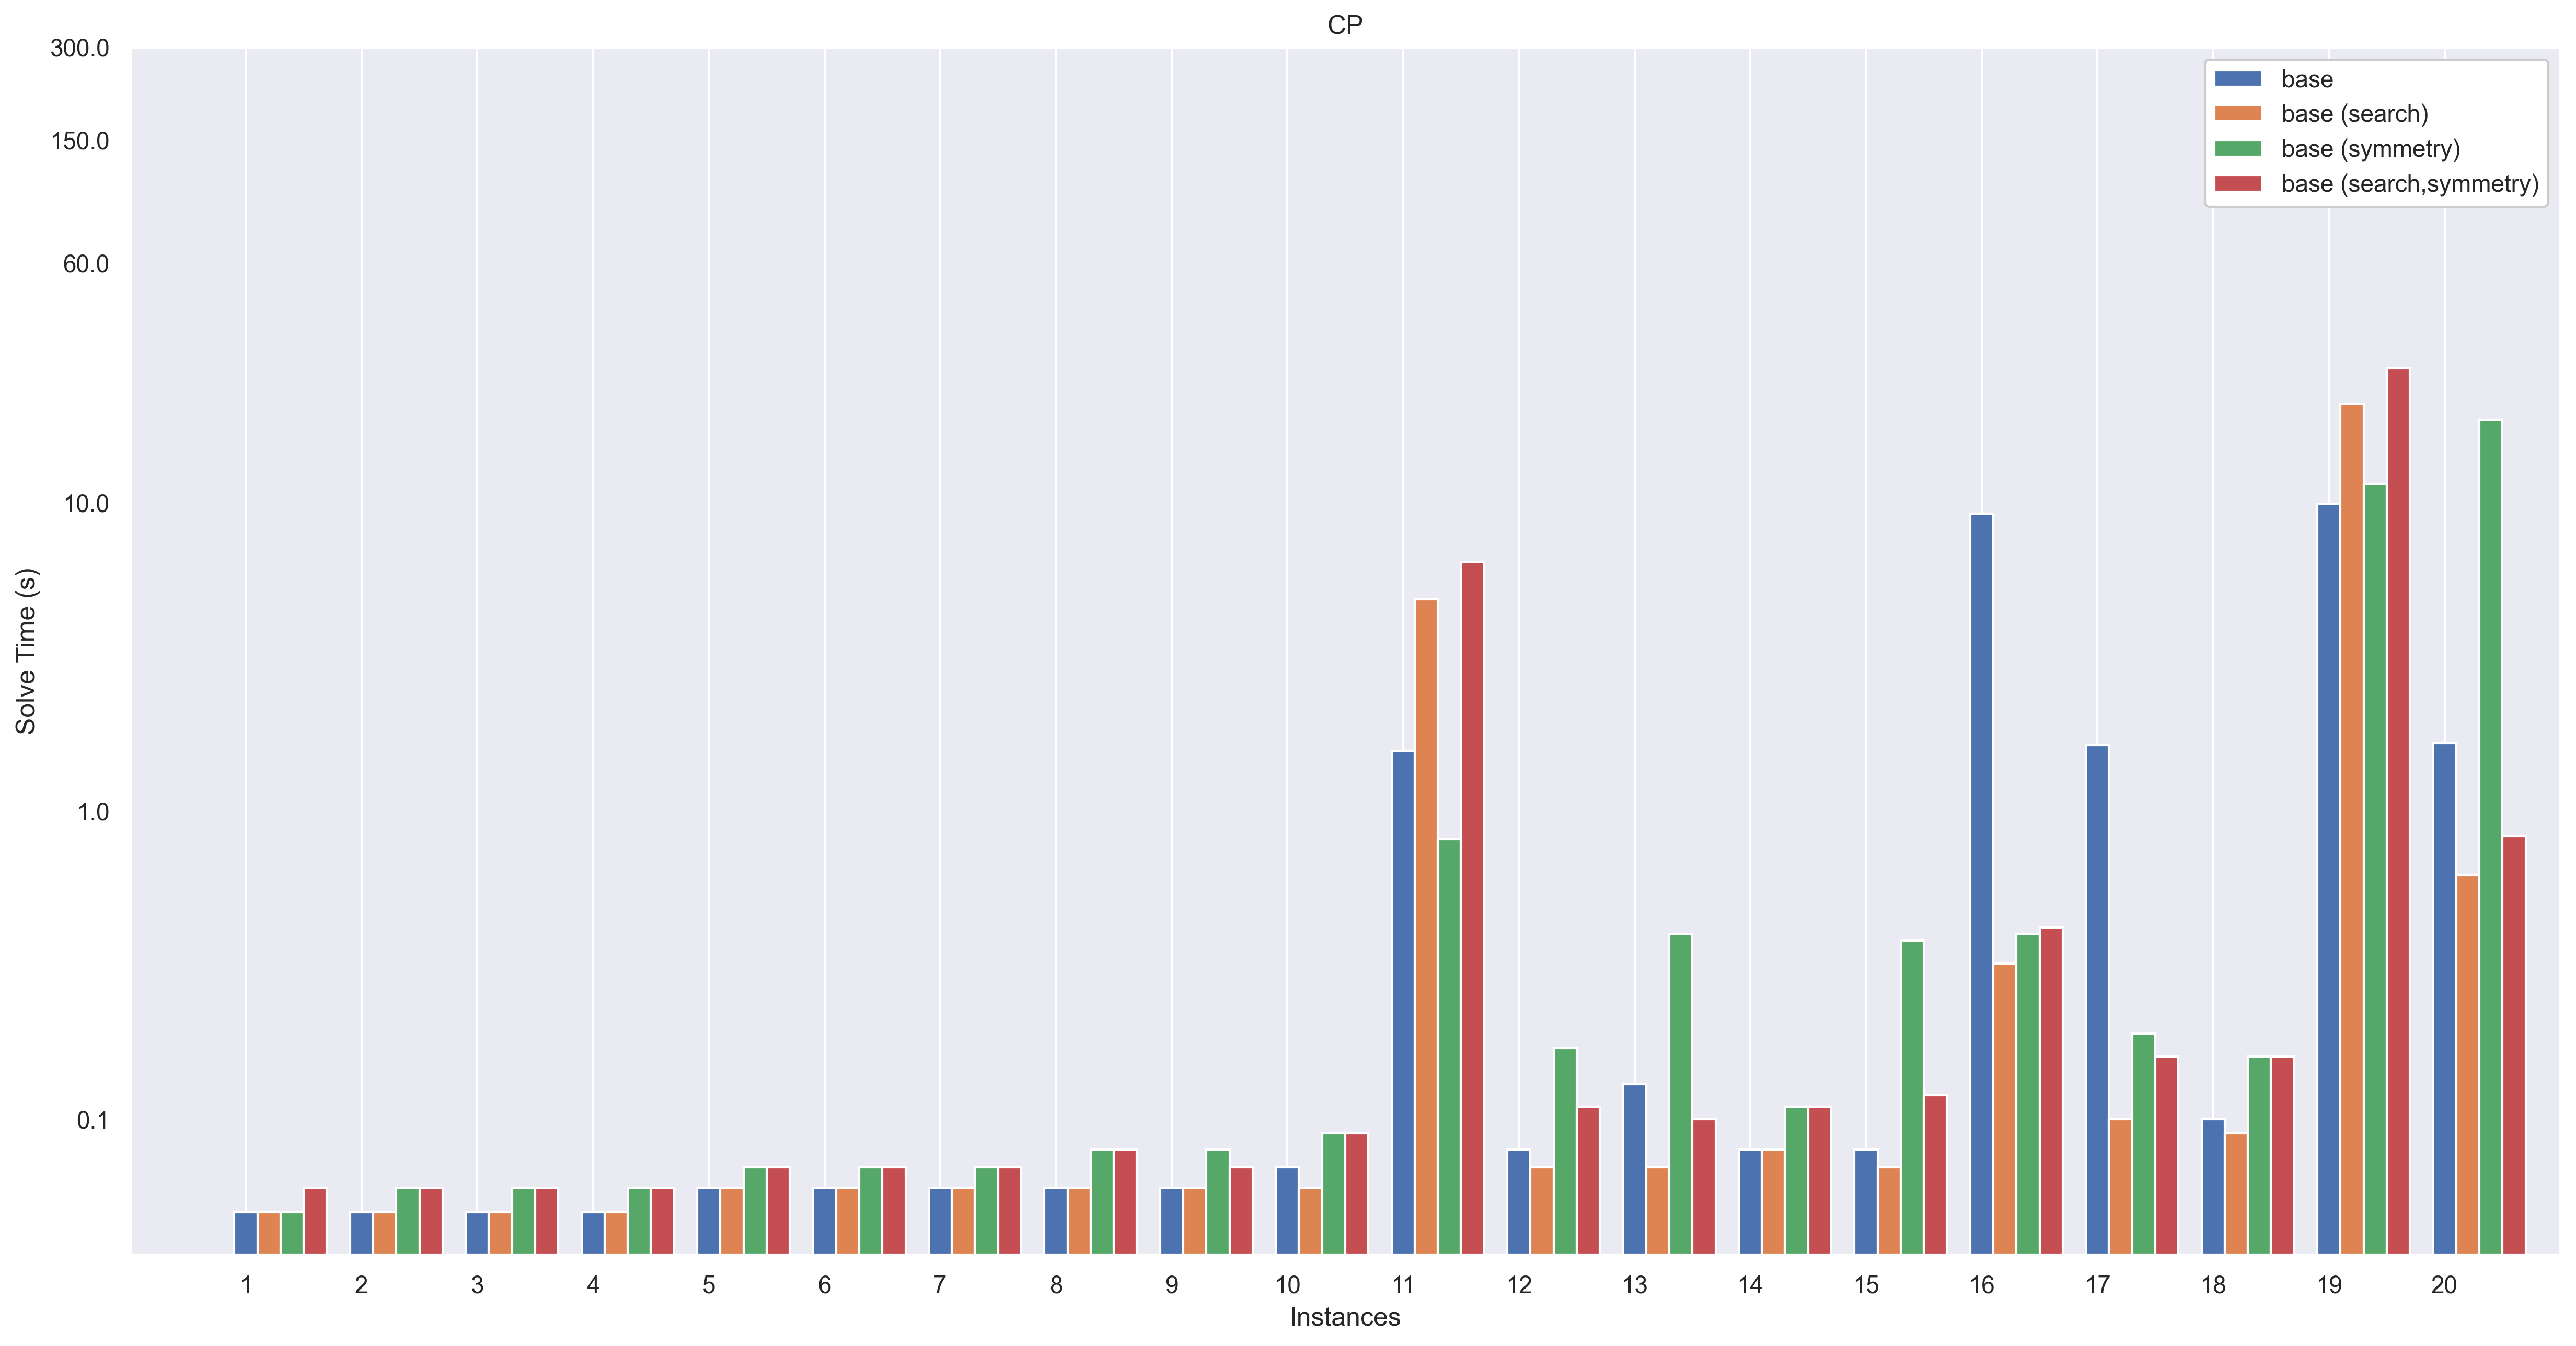
\includegraphics[width=1\textwidth]{05/results/base1.png}
      \caption{
        \colorbox{BurntOrange}{TODO missing ...}
      }
      \label{fig:SMT_results_base1}
    \end{figure}
    \begin{figure}[H]
      \centering
      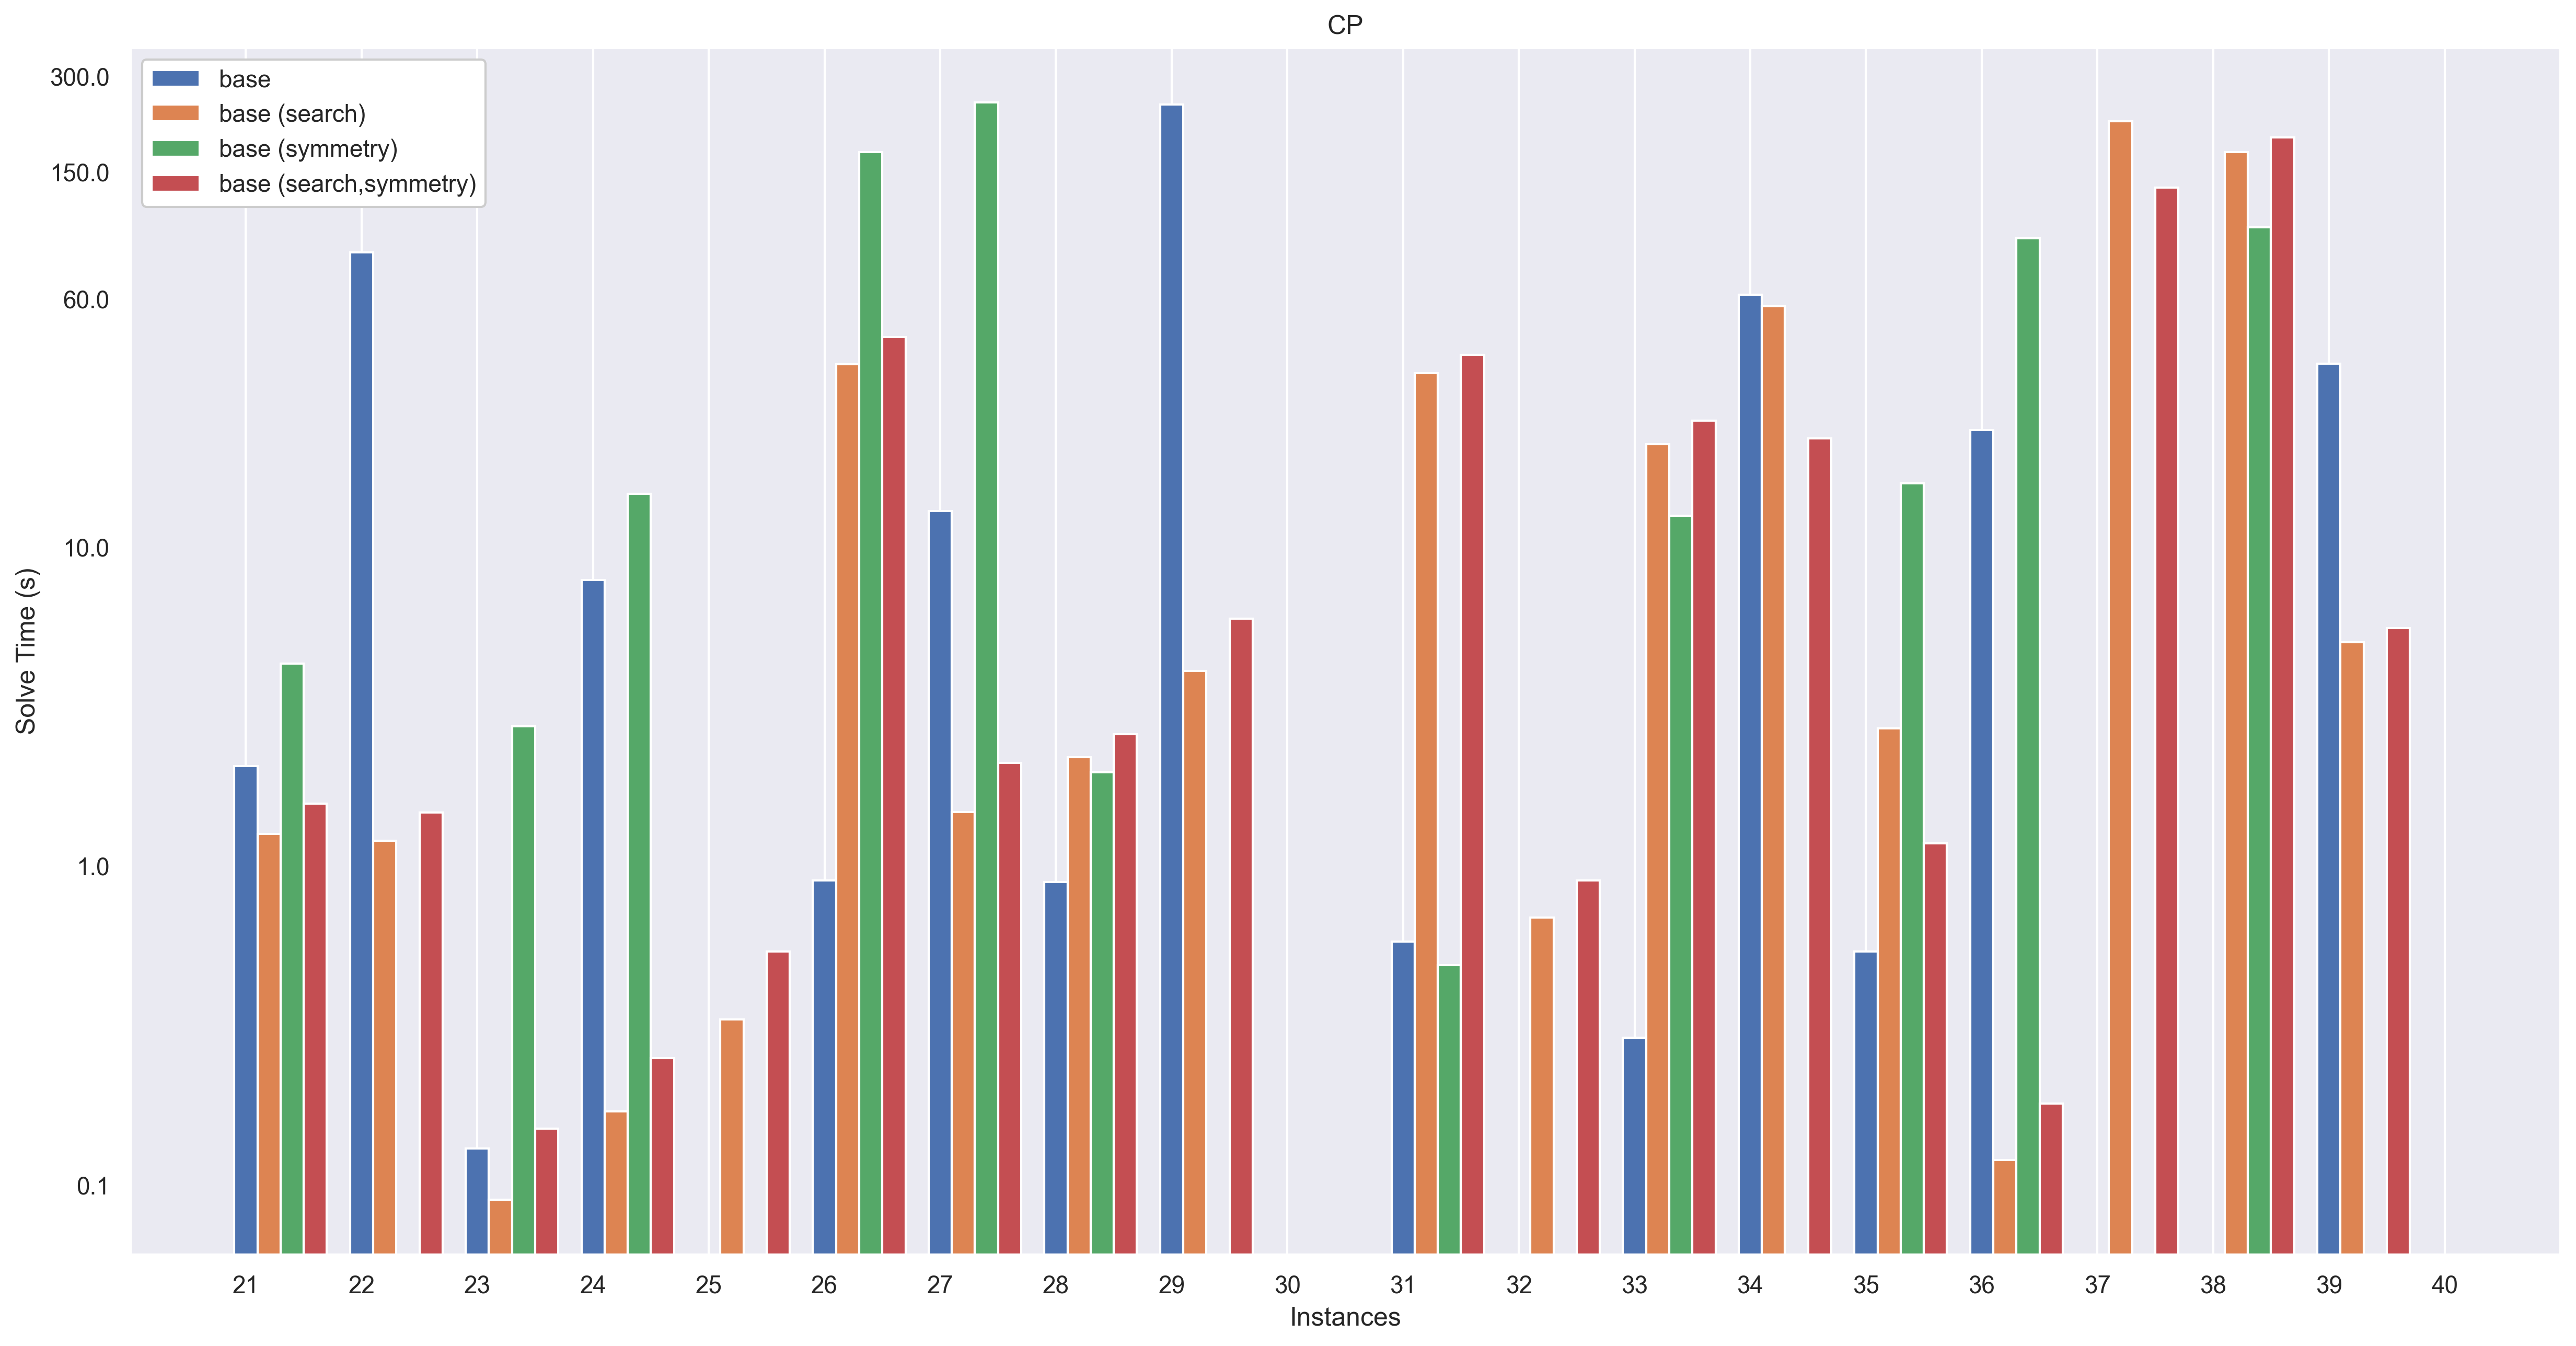
\includegraphics[width=1\textwidth]{05/results/base2.png}
      \caption{
        \colorbox{BurntOrange}{TODO missing ...}
      }
      \label{fig:SMT_results_base2}
    \end{figure}

    \colorbox{BurntOrange}{TODO missing ...} \\

    \begin{figure}[H]
      \centering
      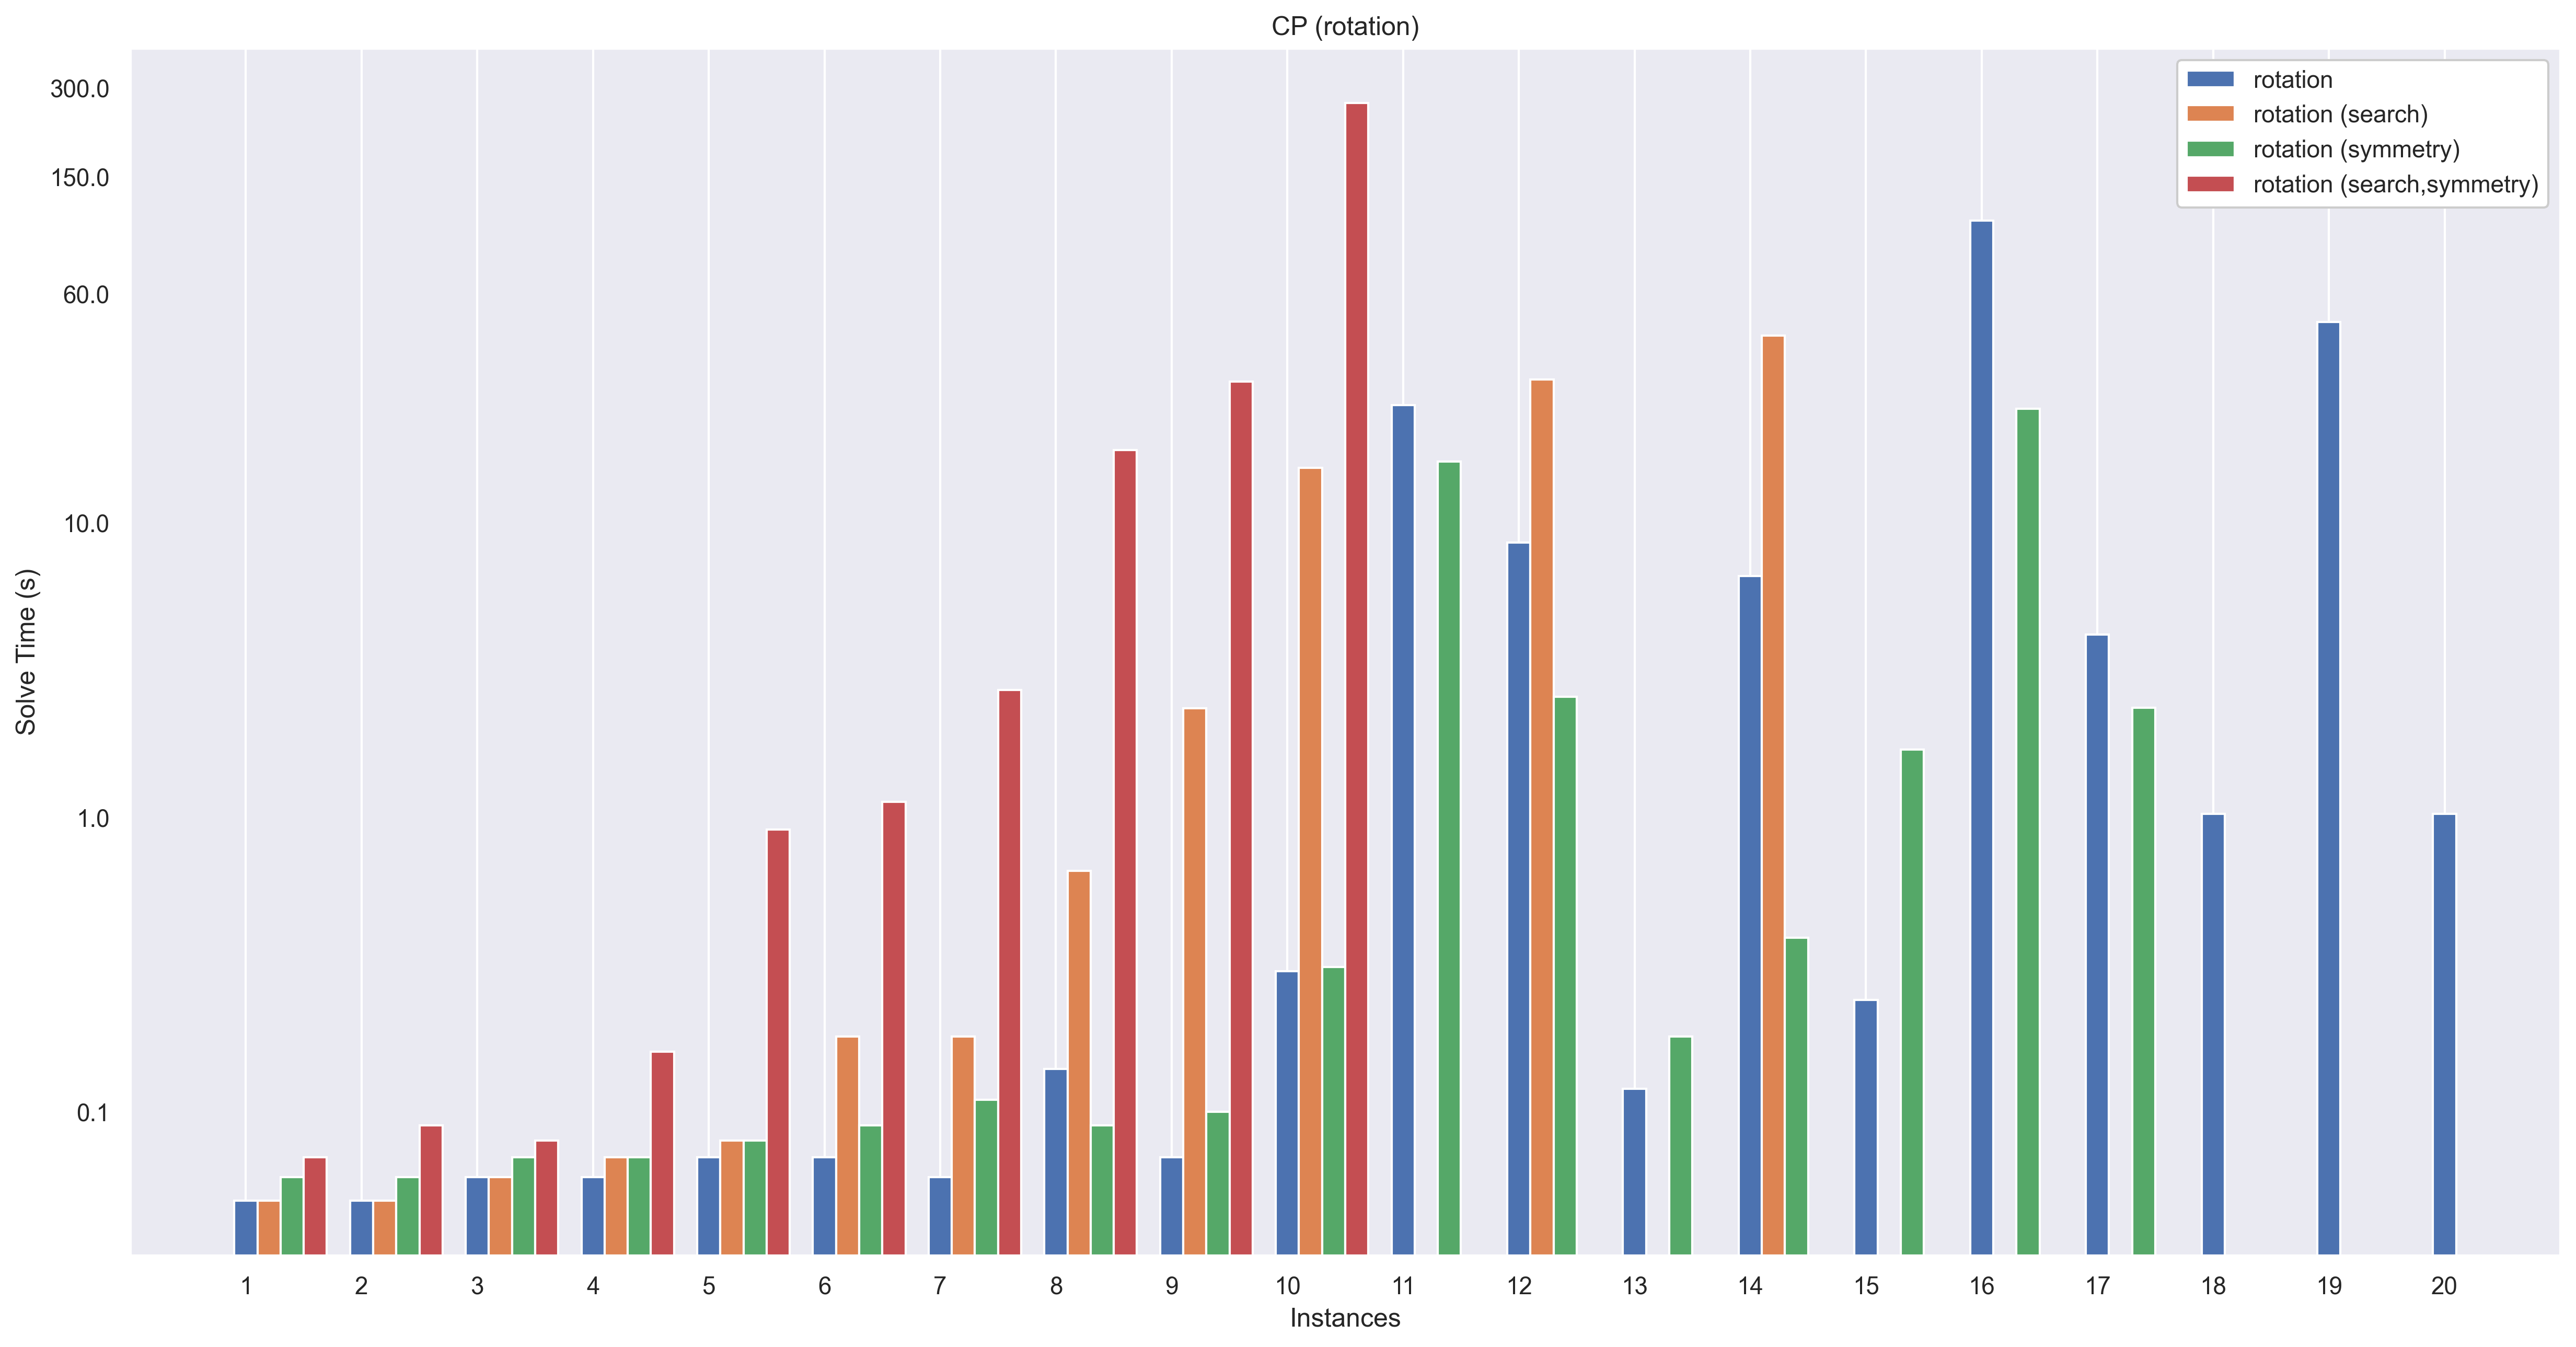
\includegraphics[width=1\textwidth]{05/results/rotation1.png}
      \caption{
        \colorbox{BurntOrange}{TODO missing ...}
      }
      \label{fig:SMT_results_rotation1}
    \end{figure}
    \begin{figure}[H]
      \centering
      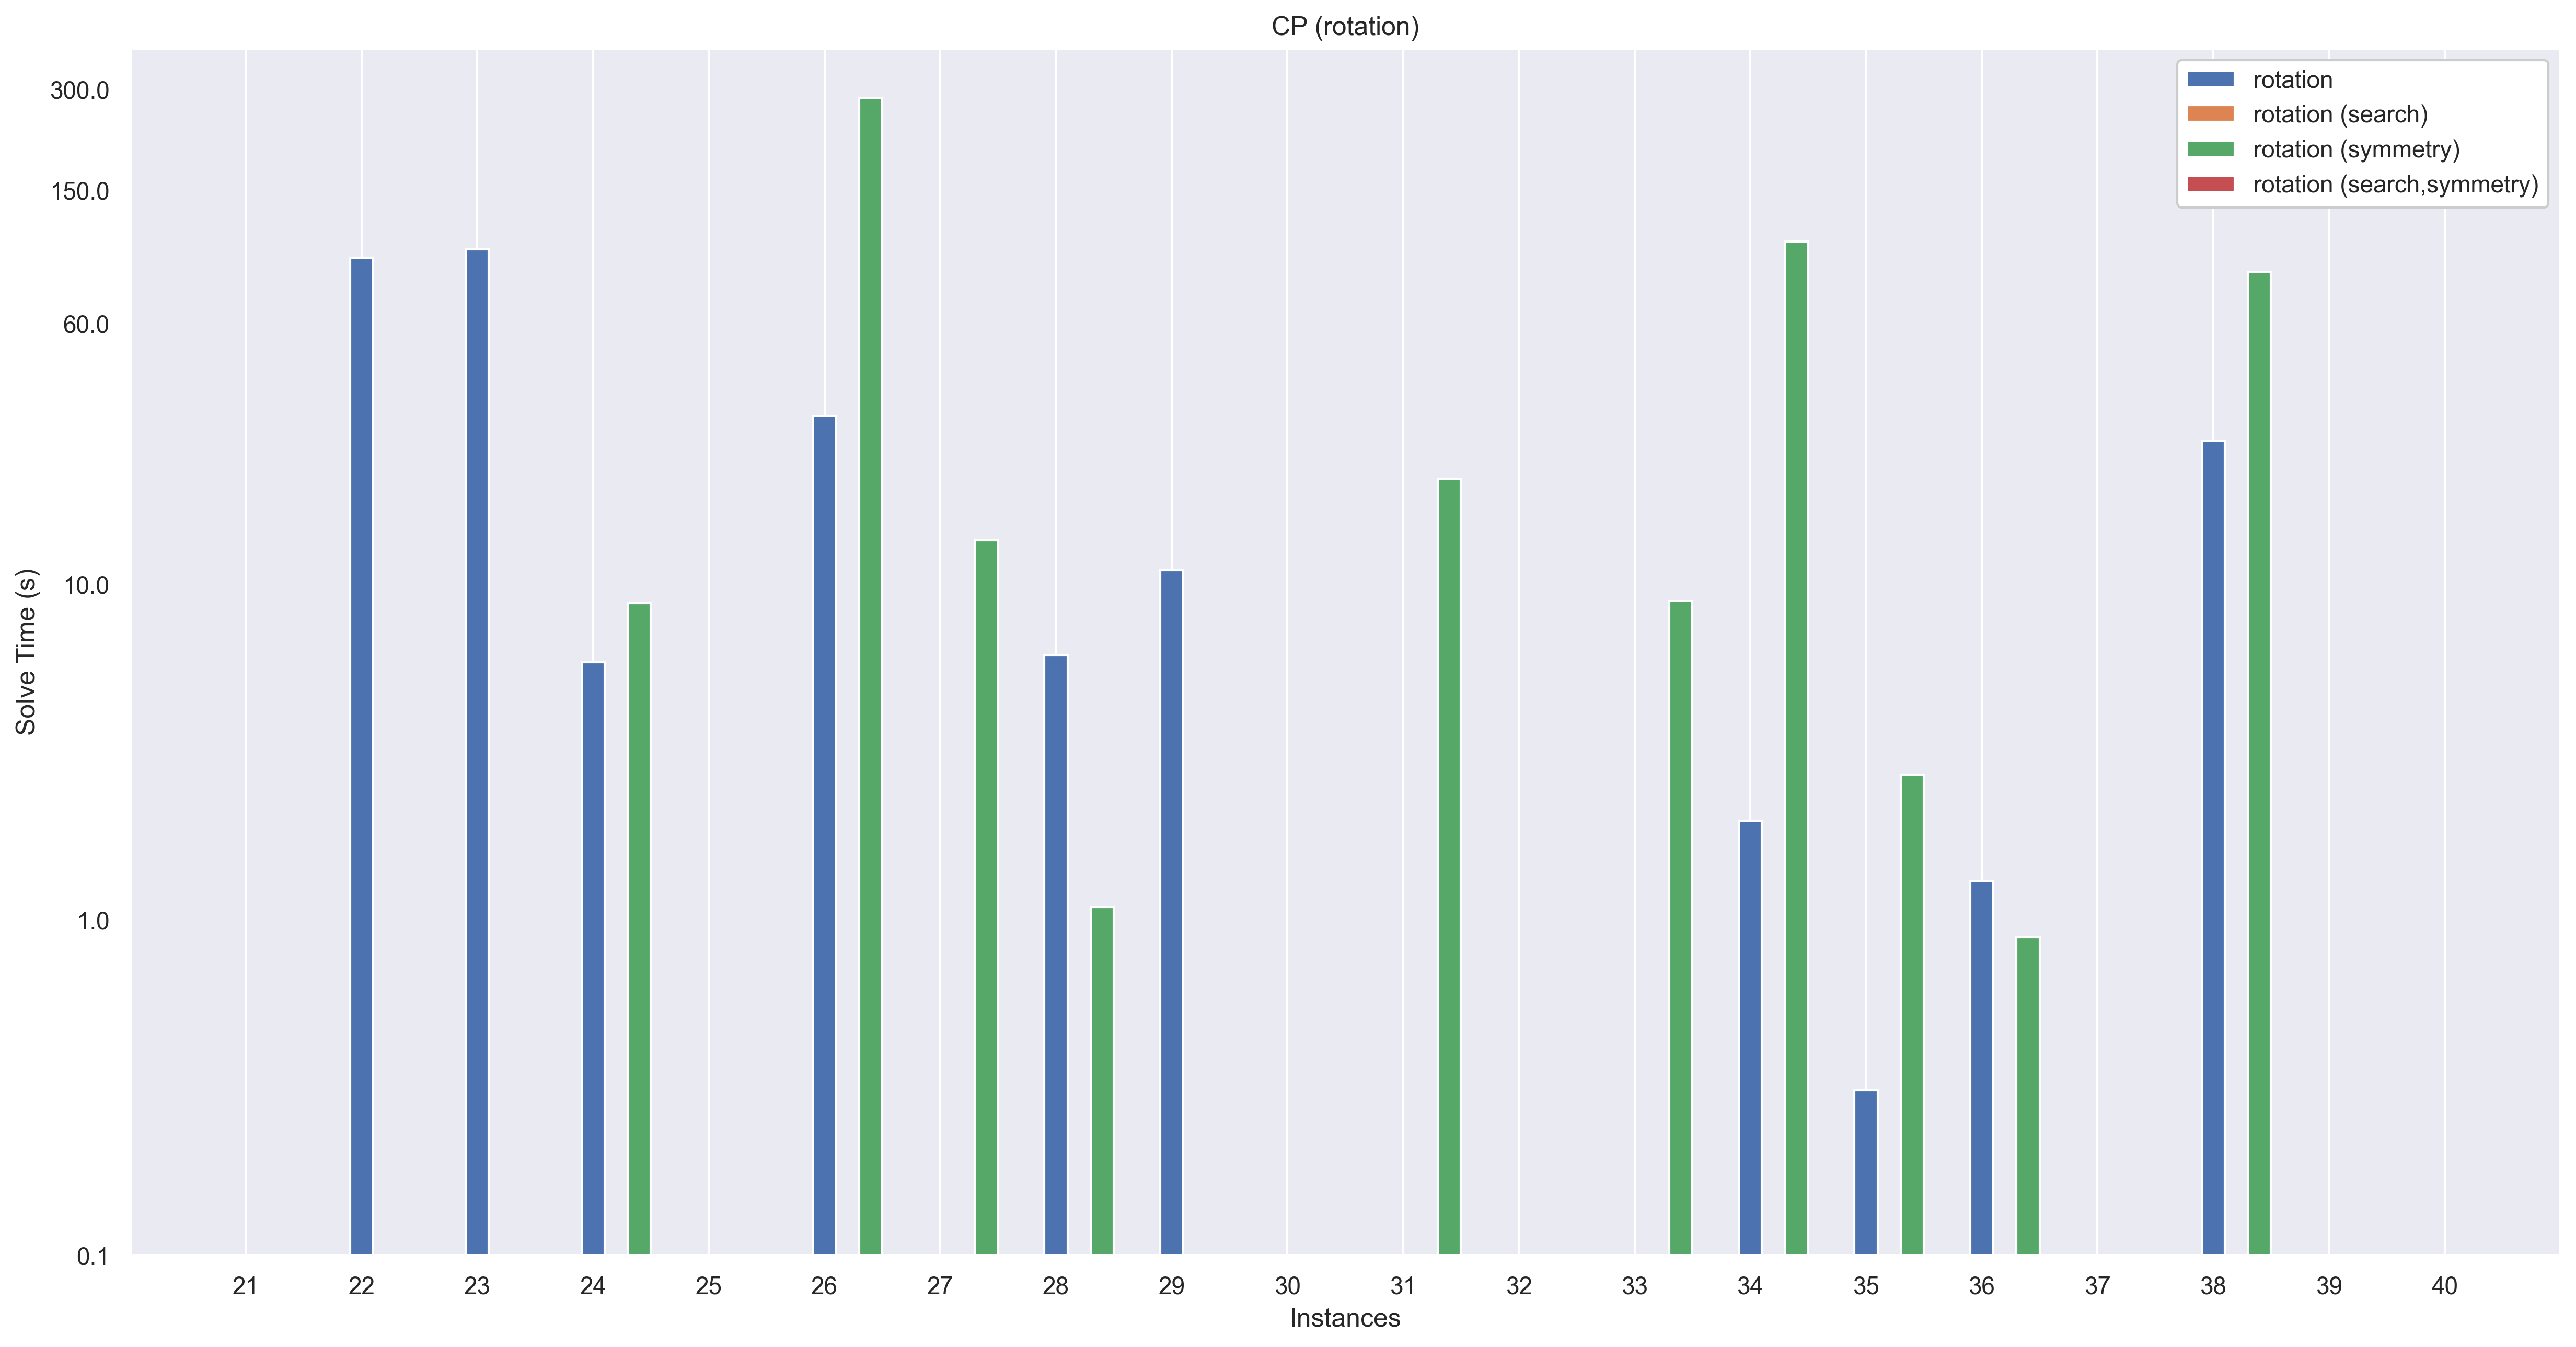
\includegraphics[width=1\textwidth]{05/results/rotation2.png}
      \caption{
        \colorbox{BurntOrange}{TODO missing ...}
      }
      \label{fig:SMT_results_rotation2}
    \end{figure}
